\chapter{Data Structures and Algorithms}
\chlabel{Data Structures and Algorithms}

In this chapter we give a description to some of the most complex
algorithms and data structures in the \GROOVE implementation. This should
help the developer to have a relatively high-level view on \GROOVE. This
description is to be considered together with the {\em javadoc} that gives
a detailed explanations on the classes / methods, that we do not reproduce
here.

\section{Storage of Graphs}
\stlabel{storage of graphs}

The tool \GROOVE manipulates a labelled transition system that may contain
a very big number of graphs as states. Space is a critical resource for the
tool, and efficient storage of graphs is essential.

There are two essential mechanisms in \GROOVE that are related to efficient
graph storage, while trying to keep an optimal time performance:
\begin{itemize}
\item a {\em delta graph} is a representation of a graph expressed by the
  changes that one should operate on some {\em basis graph} in order to
  obtain it. {\em Changes} are added and removed elements (nodes or edges).
  Delta graphs are very useful as in a labelled transition system most of
  the new graphs are generated by graph transformation, thus share lots of
  common structure with other graphs. This is the format in which graphs
  are represented in run-time;
\item a {\em graph cache} is a representation of a graph as a set of nodes
  and a set of edges with additional information in order to make graph
  processing easier. If the JVM runs out of memory, the garbage collector
  is authorised to remove cache graphs. If some computations with a graph
  are involved, then the cache is recomputed again.
\end{itemize}

On \fref{graphs} we depict the class hierarchy relative to the
representation of graphs and delta graphs in \GROOVE. On \fref{elements} is
represented partially the class hierarchy relative to graph elements
(nodes, edges). Finally, \fref{caches} gives a portion of the class
hierarchy related to graph caches. For further details, we refer to the
{\em javadoc}.
\begin{figure}[ht]
  \centering
  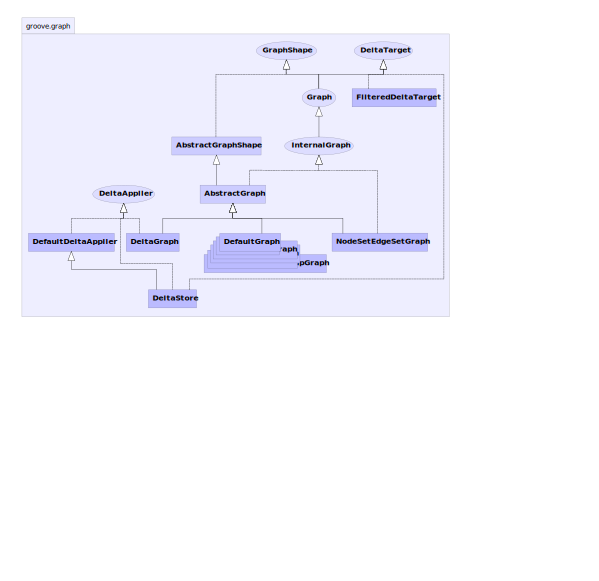
\includegraphics{fig/graphs}
  \caption{Graph related class hierarchy.}
  \flabel{graphs}
\end{figure}

\begin{figure}[ht]
  \centering
  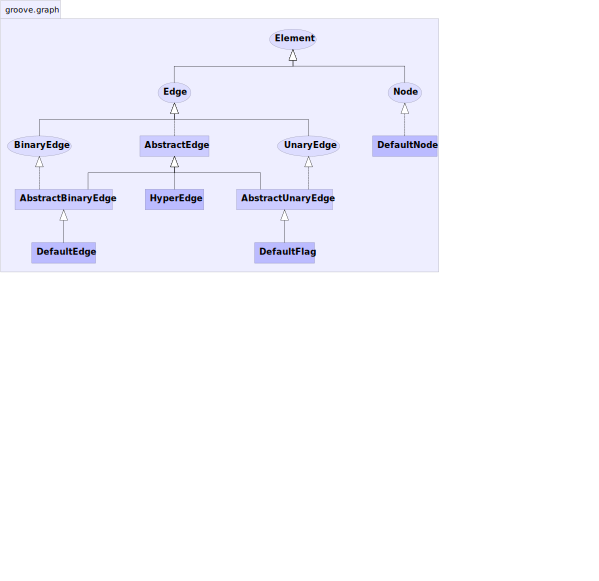
\includegraphics{fig/elements}
  \caption{Part of the class hierarchy relative to graph elements.}
  \flabel{elements}
\end{figure}

\begin{figure}[ht]
  \centering
  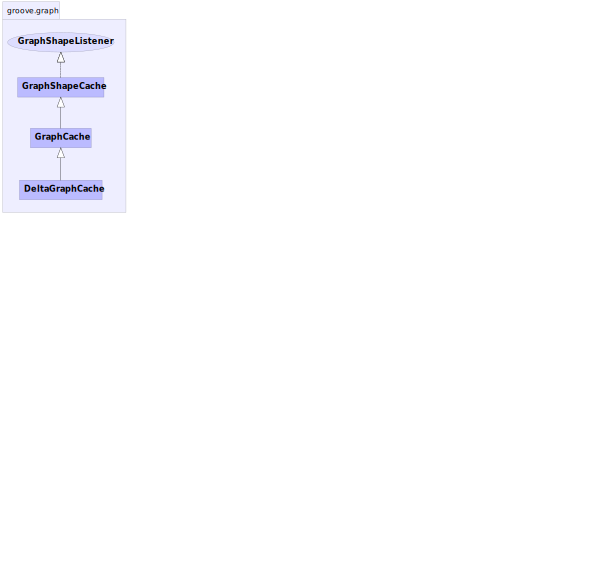
\includegraphics{fig/caches}
  \caption{Part of the class hierarchy relative to graph cache.}
  \flabel{caches}
\end{figure}

\paragraph{Delta Graph}
A {\em delta graph} is essentially a basis graph together with a set of
added elements and a set of removed elements (nodes or edges). For storage
optimisation, added and removed elements are stored into a single array,
called {\em delta array}. The basis graph can also be a delta graph.  Thus,
we can have a sequence of delta graphs, each of which is used as a basis of
the next one. Very long such sequences may result in a big loss of time
efficiency, as most of the manipulations on a graph require a node-set
edge-set based representation, which should be recomputed. Therefore, the
length of such sequences is limited to at most {\tt
  graph.DeltaGraphCache.FREEZE\_DEPTH}, currently set to $8$.
% TODO : what is a frozen delta graph ?
% TODO : make sure that it is indeed the limit

\paragraph{Graph Cache}
A graph cache is a representation of a graph that contains explicitly the
sets of nodes and edges of the graph, as well as adjacency map associating
with each node its adjacent edges, and edge label map, associating with
each label the edges wearing this label. This redundant representation
facilitates computations on a graph. 

An object of type {\tt graph.AbstractGraphShape} contains a reference to a
{\tt graph.GraphShapeCache} (in the form of a {\tt
  java.lang.ref.Reference<GraphShapeCache>} object), and it supports a {\tt
  clearCache()} operation that allows to notify the garbage collector that
the cache object can be collected in case there is a need of additional
memory.

\section{Labelled Transition System}

Remind that the \GROOVE Simulator and Generator allow to (partially)
construct the labelled transition system corresponding to some graph
grammar. Such a LTS is of the form $\mathcal S = (S, T, s_0, F)$. States in
$S$ are graphs and transitions in $T$ are of the form $(G, (P,m), H)$,
where the graphs $G,H$ are states of the labelled transition system and the
label $(P,m)$ consists of a graph production $P$ and a matching $m: L \to
G$ (with $P = (L, R)$).

The functionality of Groove related to computing and storing a Labelled
Transition System (LTS) is implemented into two packages.
\begin{itemize}
\item \texttt{lts} package for construction and storage of a labelled transition system,
\item \texttt{trans} package for computing transformations.
\end{itemize}
In what follows we describe these implementations. We start with a general
description, and then give details on the implementations. We omit the {\tt
  groove} prefix in class names (i.e. we write {\tt lts.GTS} instead of
{\tt groove.lts.GTS}).

\subsection{Interface for a Labelled Transition System}
A LTS is a graph-like structure. The interface {\tt graph.GraphShape}
defines basic graph functionality, such as adding, removing and retrieving
nodes and edges and sets of nodes and edges, etc. The interface {\tt
  lts.LTS} (\fref{lts-interface}) extends the interface {\tt
  graph.GraphShape} with the notion of start and final states and with the
method

\smallskip\noindent%
{\tt boolean isOpen(State state);}

\noindent
A state of a LTS is considered {\em open} if not all outgoing transitions have
not been explored.

\begin{figure}[ht]
  \centering
  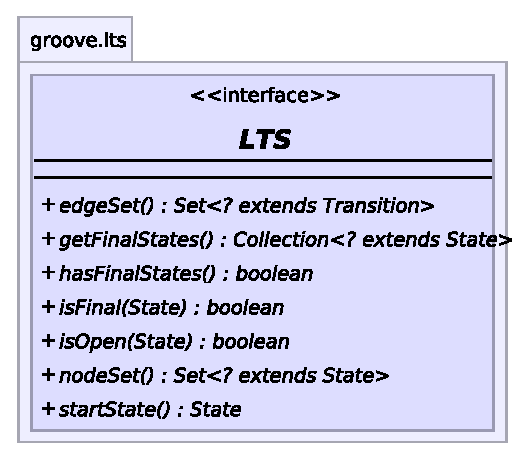
\includegraphics[scale=0.8]{fig/LTS}
  \caption{The interface {\tt lts.LTS}.}
  \flabel{lts-interface}
\end{figure}


\paragraph{States and Transitions of a Labelled Transition System}

The {\tt lts} package provides the hierarchy of states and
transitions of an LTS depicted on \fref{states and transitions}.

\begin{figure}[ht]
  \centering
  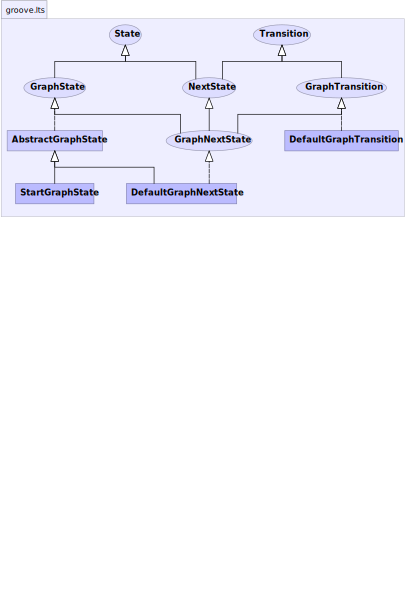
\includegraphics{fig/states-and-transitions}
  \caption{States and transitions class hierarchy for a LTS.}
  \flabel{states and transitions}
\end{figure}

The interface {\tt lts.NextState} combines a state and a transition. It is
intended to represent a state together with one of its incoming
transitions. The interface {\tt lts.GraphState}, {\tt lts.GraphTransition}
and {\tt lts.GraphNextState} specialise a state, a transition and a ``next
state'' for labelled transition systems which states are graphs and which
transitions represent direct derivations. The classes {\tt
  lts.DefaultGraphTransition}, {\tt lts.DefaultGraphNextState} and {\tt
  lts.StartGraphState} are the implementations of these interfaces. On
\fref{graphstate} we present in more detail the functionality provided by
the interface {\tt lts.GraphState}. As one can see from this figure, a {\tt
  lts.GraphState} knows its outgoing transitions. The {\tt setClosed()}
method closes the state, forbidding to add more outgoing transitions to it.

\begin{figure}[ht]
  \centering
  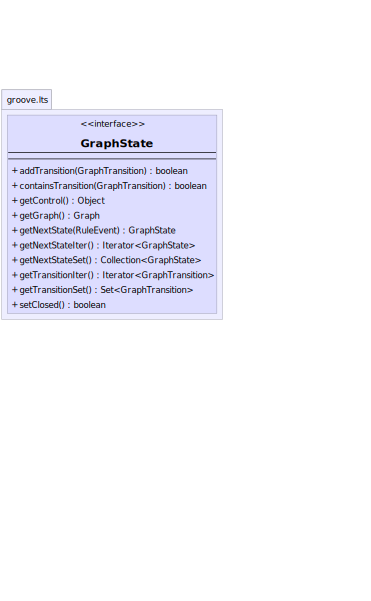
\includegraphics{fig/GraphState}
  \caption{Partial description of the interface {\tt lts.GraphState}.}
  \flabel{graphstate}
\end{figure}

\subsection{Storing a Labelled Transition System}

A labelled transition system is stored in an object of class {\tt lts.GTS}
(for Graph Transition System, i.e. transition system which states are
graphs), which implements {\tt lts.LTS}.

Let us first give an intuitive explanation of the way a LTS is stored.
Given an LTS $\mathcal S = (S, T, s_0)$, a {\em spanning tree} of $\mathcal
S$ is a tree whose set of nodes is $S$, has $s_0$ as a root, and whose
arrows are transitions in $T$ (see \fref{spanning tree} for an example of a
spanning tree). That is, a spanning tree contains all nodes of a LTS, but
not all transitions. However, if for any node we have sufficient
information allowing to reconstruct its outgoing transitions, then we can
easily reconstruct the whole LTS from its spanning tree. Storing a LTS as
one of its spanning trees allows to save space if we can store the missing
transitions in an efficient way. Now, a spanning tree can be completely
defined by its root and its set of nodes, if any node contains also its
unique (in the spanning tree) incoming arrow. This possibility is offered
by the interface {\tt lts.GraphNextState}.  We will see in the next section
how the possibility of efficient storage of an LTS by its spanning tree is
explored during the construction of an LTS.

\begin{figure}[ht]
  \centering
  \includegraphics{fig/spanning-tree}
  \caption{A labelled transition system on the left and one of its spanning trees on the right.}
  \flabel{spanning tree}
\end{figure}

% \paragraph{Efficient Storage of Transitions in an LTS}
% As we mentioned previously, transitions of a GTS are stored as outgoing
% transitions by the states of the GTS. Therefore, it is not necessary to
% store the source state of a transition. The interface {\tt
%   lts.GraphOutTransition} describes transitions that do not know their
% source state. Its implementation {\tt lts.DefaultGraphOutTransition} thus
% defines a transition as a {\tt trans.RuleEvent} and a {\tt
%   lts.TargetState}. A {\tt trans.RuleEvent} is essentially a graph
% production and a host graph together with the image of the anchor of the
% left-hand side of the rule into the host graph. 

% \paragraph{Efficient Storage of States in an LTS}
% As described in \stref{storage of graphs}, several techniques are employed
% for efficient storage of graphs. Further optimisations can be done when
% graphs are the states of a LTS. A {\tt lts.GTS} stores its set of states as
% a set of objects of type {\tt lts.DerivedGraphState} (except for the start
% state).  As shown on \fref{states and transitions}, a {\tt
%   lts.DerivedGraphState} extends a {\tt graph.DeltaGraph}. Remind that a
% {\tt graph.DeltaGraph} stores a basis graph as well as an array of modified
% -- added and removed -- elements.  A {\tt lts.DerivedGraphState} contains
% information on its predecessor state in the spanning tree of the LTS and
% the corresponding incoming transition. The predecessor state is the basis
% graph. This transition contains the rule and the matching into the basis
% graph, thus removed elements can be deduced from it. Therefore, the delta
% array of a {\tt lts.DerivedGraphState} stores only the elements added to
% basis graph while performing the transition. These elements are also called
% {\em co-anchor image}: the image of the elements of the right-hand
% side of the rule that are new (w.r.t. the left-hand side).

\subsection{Constructing a Labelled Transition System}

The construction of a LTS is always done according to some exploration
strategy. In practise, the LTS corresponding to some graph grammar is often
infinite. Therefore, the strategy defines how to generate a portion of it
(e.g. depth-first, breadth-first). The strategy interface is given on
\fref{ExploreStrategy}.

\begin{figure}[ht]
  \centering
  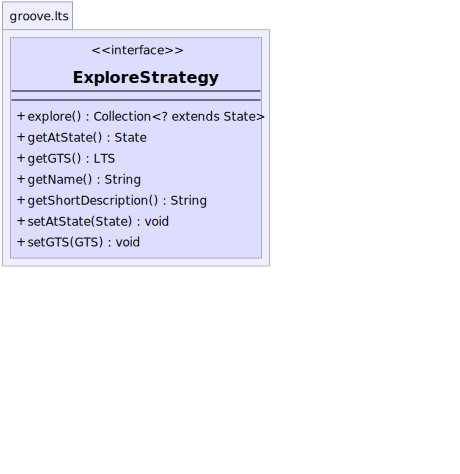
\includegraphics[scale=0.8]{fig/ExploreStrategy}
  \caption{The {\tt lts.ExploreStrategy} interface.}
  \flabel{ExploreStrategy}
\end{figure}

It allows to set the exploration at a given state ({\tt setAtState}) and to
make an exploration. For a list of the implemented strategies the reader is
invited to consult the {\em javadoc}.

The class {\tt lts.StateGenerator} that provides basic functionality for
generating new states in of a {\tt lts.GTS}, and is used as an interface by
the strategies. On \fref{StateGenerator} is depicted a partial view of the
functionality provided by this class.

\begin{figure}[ht]
  \centering
  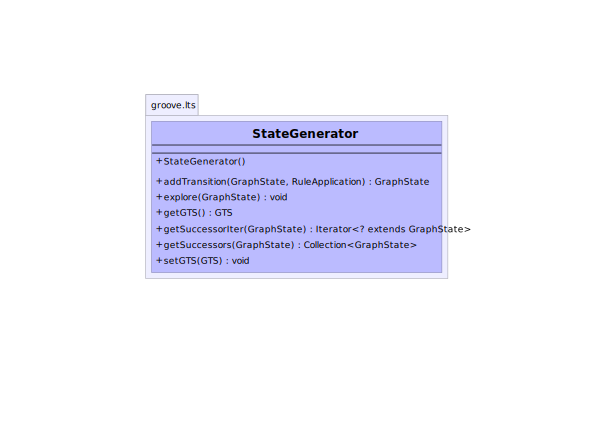
\includegraphics{fig/StateGenerator}
  \caption{Partial description of the class {\tt lts.StateGenerator}.}
  \flabel{StateGenerator}
\end{figure}

The method {\tt addTransition} adds a new transition to the associated GTS
(here a GTS) for the given source node and a {\tt trans.RuleApplication}.
The method {\tt explore} adds all (not already present) transitions to the
given state. Finally, the class gives to possibility to retrieve, or
iterate over, the successor states of a given state. 

% TODO
% We would like to describe here briefly different optimisation methods used
% while constructing the LTS.



% One can see that this class gives the possibility to compute the target
% state for some rule application, to add a transition to a LTS, or compute
% or iterate over all (already computed) successors of a given state. The
% protected method {\tt getConfluentTarget(RuleApplication)} is used for
% computing a successors state. It tries to derive the successor state
% walking around three sides of a confluent diamond instead of computing the
% state directly. When it is not possible, a {\tt lts.StateGenerator} uses a
% so called {\tt trans.Deriver} for performing the actual transformation.

% We give here only a brief description of derivers. More information can be
% find in the {\em javadoc}.

% On \fref{graph transitions} we show some hierarchies of classes used for
% representing a rule application.

% \begin{figure}[ht]
%   \centering
%   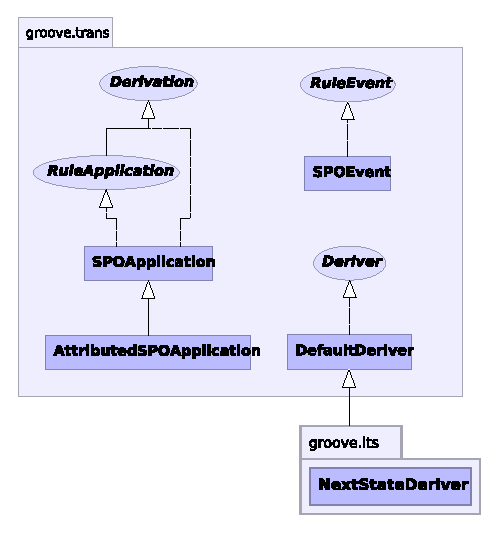
\includegraphics{fig/graph-transitions}
%   \caption{Hierarchy of classes for rule application.}
%   \flabel{graph transitions}
% \end{figure}

% Relative to the construction of the labelled transition system is the class
% {\tt lts.NextStateDeriver}. This is an implementation of a {\tt
%   trans.Deriver} that guarantees that newly generated graphs will be of
% type {\tt lts.DefaultNextState}. These is the run-time type of states of a
% {\tt lts.GTS}. Thus, a {\tt lts.StateGenerator} uses a {\tt
%   lts.NextStateDeriver} for computing graph derivations.


